\documentclass{beamer}

%\usetheme[framenumber,totalframenumber]{UniversiteitGent}
%\usetheme[faculty=di,framenumber,totalframenumber]{UniversiteitGent}
%\usetheme[faculty=we,usecolors,framenumber,totalframenumber]{UniversiteitGent}
\usetheme[language=english,framenumber,totalframenumber]{AlleghenyCollege}

\title{Introduction to Computer Science I}
\author{Janyl Jumadinova \\ January 17, 2018}

\long\def\omitit#1{}

\begin{document}

\begin{frame}
  \titlepage
\end{frame}

%%%%%%%%%%%% Slide %%%%%%%%%%%%%%%%%%%%%%%%%%%%%%%%%%%%%%%%%%%%%%%%%%%
\begin{frame}
  \frametitle{Keep in Touch}
	\begin{itemize}
        \item Email
		\item Office hours
		\item Course website (\url{http://cs.allegheny.edu/sites/jjumadinova/teaching/111})
		\item Teaching assistants (\url{http://www.cs.allegheny.edu/teaching/teachingassistants/})
		\item Sakai (\url{https://sakai.allegheny.edu/})
		\item Slack channel (more on this later) (\url{https://cs111s2018.slack.com/})
		\item Github (more on this later) (\url{https://github.org/})
    \end{itemize}
\end{frame}
%%%%%%%%%%%% Slide %%%%%%%%%%%%%%%%%%%%%%%%%%%%%%%%%%%%%%%%%%%%%%%%%%%

\begin{frame}
  \frametitle{What will we explore in this class?}
		\pause
      \begin{itemize}
        \item Algorithms
        \item Software 
        \item Programming Languages - Java
        \item Applications of computer science \pause
        \begin{itemize}
        	\item DNA manipulation
        	\item Graphics
        	\item Robotics 
        	\item Music
    	\end{itemize}
    \end{itemize}
\end{frame}

%%%%%%%%%%%% Slide %%%%%%%%%%%%%%%%%%%%%%%%%%%%%%%%%%%%%%%%%%%%%%%%%%%
\begin{frame}
  \frametitle{Computer Science Involves More than Programming!}
	\begin{itemize}
		\item People
        \item Teams
        \item Writing
        \item Speaking
    \end{itemize}
\end{frame}

%%%%%%%%%%%% Slide %%%%%%%%%%%%%%%%%%%%%%%%%%%%%%%%%%%%%%%%%%%%%%%%%%%
\begin{frame}
  \frametitle{Highlights of this course}
    \begin{itemize}
        \item Class Activities \pause
        \item Laboratory Sessions \pause
        \item Practical Sessions (Fridays) \pause
        \item Challenging Programming \pause
		\item Group Projects \pause
		\item Fun Presentations \pause
		\item Real-world Software Tools \pause
		\item New Friends and Colleagues
    \end{itemize}

\end{frame}

%%%%%%%%%%%% Slide %%%%%%%%%%%%%%%%%%%%%%%%%%%%%%%%%%%%%%%%%%%%%%%%%%%
\begin{frame}
  \frametitle{}
	\begin{block}{
		\Huge{What is Computer Science?}}
    \end{block}
\end{frame}
%%%%%%%%%%%% Slide %%%%%%%%%%%%%%%%%%%%%%%%%%%%%%%%%%%%%%%%%%%%%%%%%%%
\begin{frame}
  \frametitle{What is Computer Science?}
  A quote from a famous computer scientist:
\emph{``Computer Science is no more about computers 
than astronomy is about telescopes''}
Edsger Dijkstra (1930 – 2002)
		 \begin{center}
    			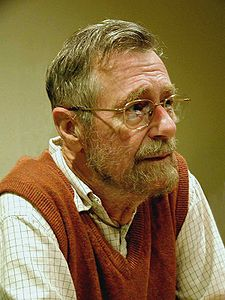
\includegraphics[scale=0.25]{images/d}
    	\end{center}
\end{frame}

%%%%%%%%%%%% Slide %%%%%%%%%%%%%%%%%%%%%%%%%%%%%%%%%%%%%%%%%%%%%%%%%%%
\begin{frame}
  \frametitle{What is Computer Science?}
	\begin{itemize}
		\item A \textcolor{blue}{computation} is a sequence of well-defined operations that lead from an initial starting point to a desired final outcome
    \end{itemize}
    \pause
    \begin{block}{\centering \Large{Computer science is the study of computation}}
    \end{block}
\end{frame}
%%%%%%%%%%%% Slide %%%%%%%%%%%%%%%%%%%%%%%%%%%%%%%%%%%%%%%%%%%%%%%%%%%
\begin{frame}
  \frametitle{}
  Computer science is the study of computation
  \pause
  	\begin{itemize}
		\item investigating problems that can be solved computationally \pause
		\item programming languages used to describe computations \pause
		\item machines that carry out computations \pause
		\item theoretical limits of computation (what is or is not computable) \pause
		\item \textbf{computational solutions to problems in math, science, medicine,  business, education, journalism, ...} \pause
    \end{itemize}
    
Computers play a key role
\end{frame}

%%%%%%%%%%%% Slide %%%%%%%%%%%%%%%%%%%%%%%%%%%%%%%%%%%%%%%%%%%%%%%%%%%
\begin{frame}
  \frametitle{What field has ...?}
  \begin{itemize}
		\item The best-rated job, and 5 of the top 10 highest paid, highest growth jobs? 

 		\item Shown strong job growth?

 		\item A severe shortage in college graduates?
    \end{itemize}
    \vspace{0.3in}
    \pause
    \centering {\huge{\textcolor{red}{Computer Science!}}}
\end{frame}
%%%%%%%%%%%% Slide %%%%%%%%%%%%%%%%%%%%%%%%%%%%%%%%%%%%%%%%%%%%%%%%%%%
\begin{frame}
  \frametitle{}
\begin{center}
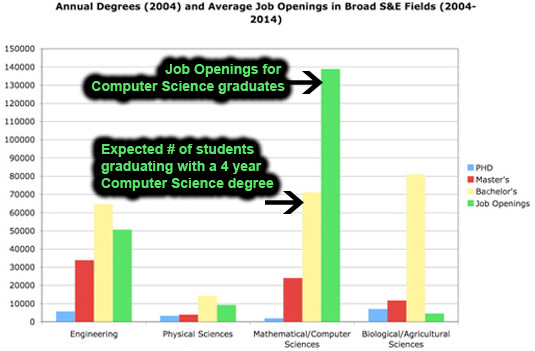
\includegraphics[scale=0.55]{images/jobs3}
\end{center}
\end{frame}
%%%%%%%%%%%% Slide %%%%%%%%%%%%%%%%%%%%%%%%%%%%%%%%%%%%%%%%%%%%%%%%%%%
\begin{frame}
  \frametitle{}
\begin{center}
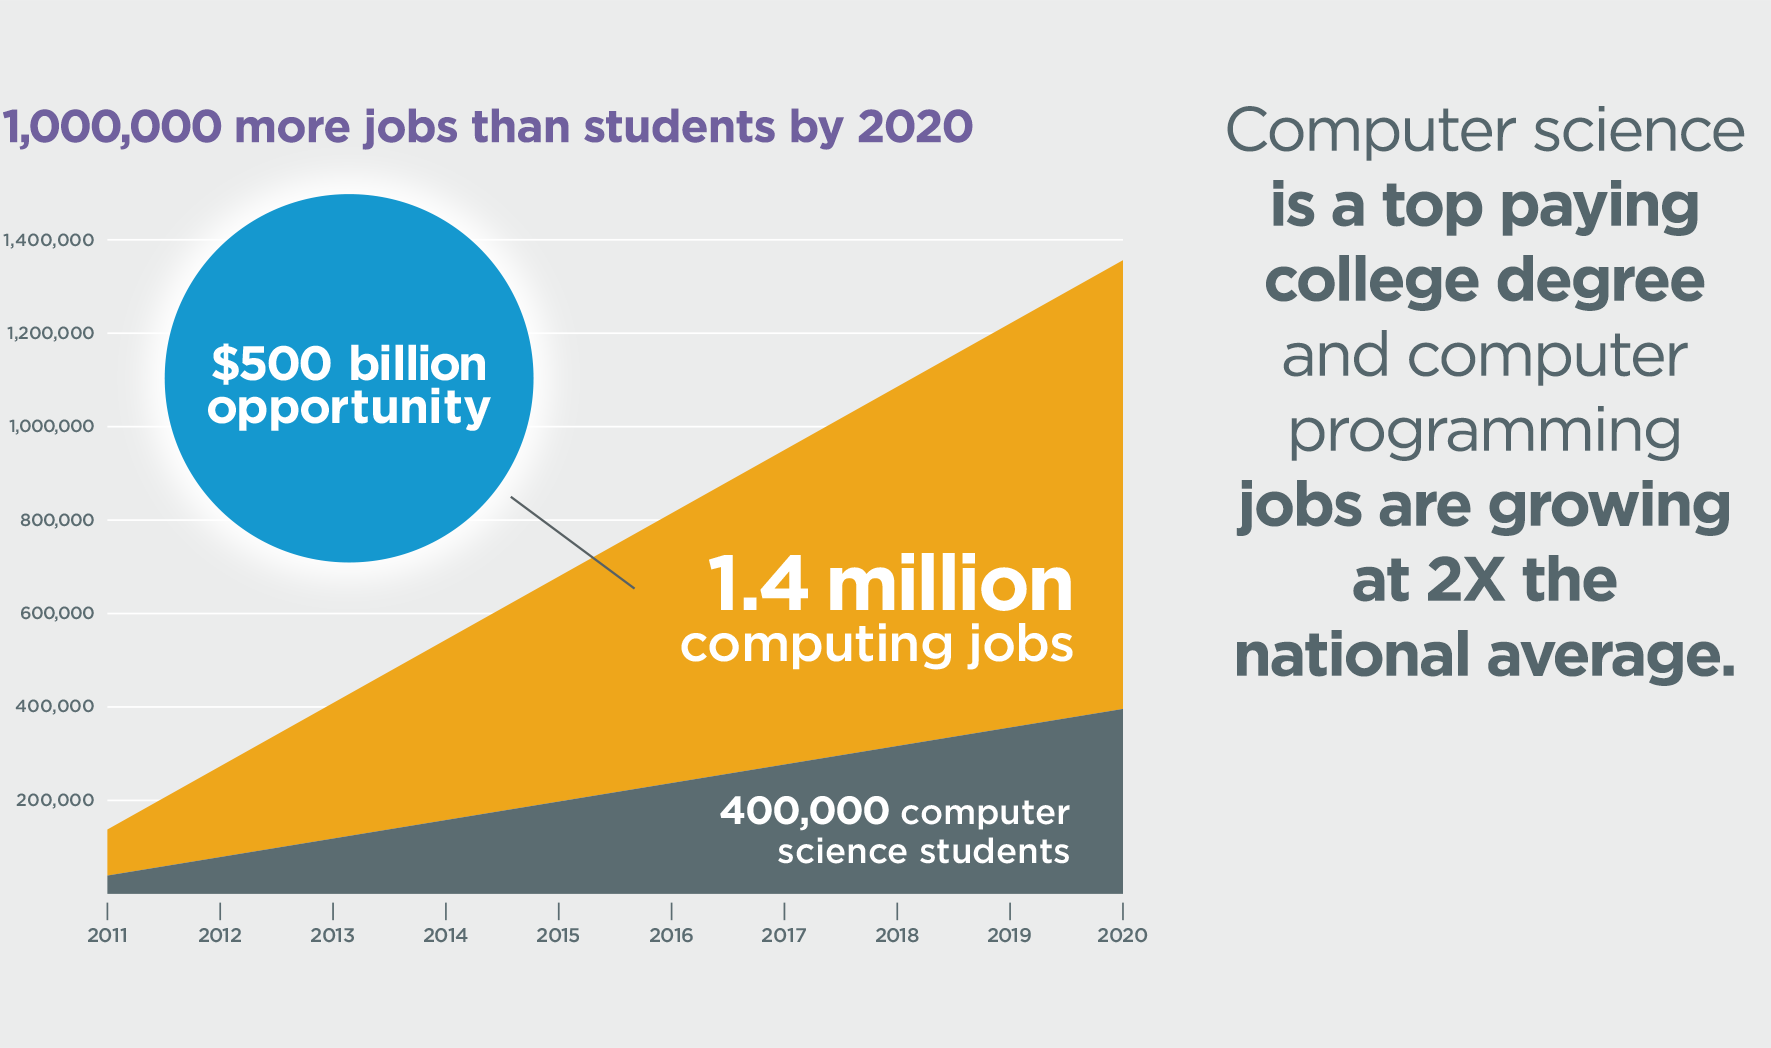
\includegraphics[scale=0.4]{images/jobs}
\end{center}
\end{frame}
%%%%%%%%%%%% Slide %%%%%%%%%%%%%%%%%%%%%%%%%%%%%%%%%%%%%%%%%%%%%%%%%%%
\begin{frame}
  \frametitle{}
\begin{center}
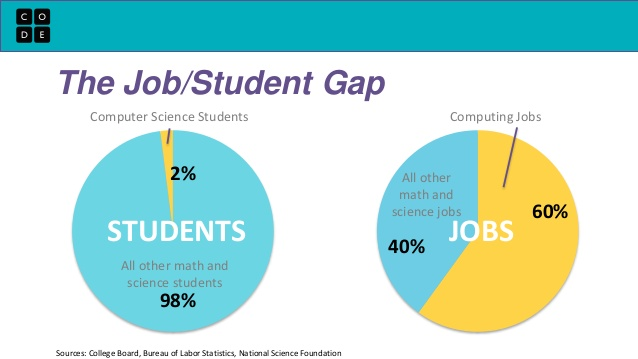
\includegraphics[scale=0.5]{images/jobs1}
\end{center}
\end{frame}

%%%%%%%%%%%% Slide %%%%%%%%%%%%%%%%%%%%%%%%%%%%%%%%%%%%%%%%%%%%%%%%%%%
\begin{frame}
  \frametitle{}
\begin{center}
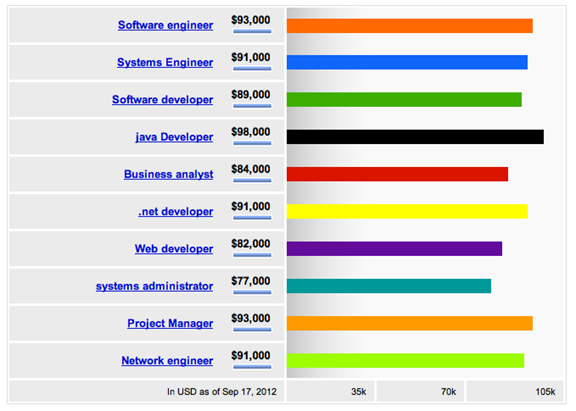
\includegraphics[scale=0.7]{images/job2}
\end{center}
\end{frame}
%%%%%%%%%%%% Slide %%%%%%%%%%%%%%%%%%%%%%%%%%%%%%%%%%%%%%%%%%%%%%%%%%%
\begin{frame}
  \frametitle{Applications of Computer Science}
  \begin{itemize}
		\item No Lab this week
		\item Practical session on Friday
    \end{itemize}
\end{frame}
 %%%%%%%%%%%% Slide %%%%%%%%%%%%%%%%%%%%%%%%%%%%%%%%%%%%%%%%%%%%%%%%%%%
\begin{frame}
  \frametitle{}
\begin{center}

\includegraphics[scale=0.3]{images/calm}
\end{center}
\end{frame}
%%%%%%%%%%%% Slide %%%%%%%%%%%%%%%%%%%%%%%%%%%%%%%%%%%%%%%%%%%%%%%%%%%

\end{document}
